% Chapter Template

\chapter{Infraestructura} % Main chapter title

\label{Chapter3} % Change X to a consecutive number; for referencing this chapter elsewhere, use \ref{ChapterX}

En este capítulo se detallarán las herramientas base empleadas en la realización de este trabajo.

%----------------------------------------------------------------------------------------
%	SECTION Hardware
%----------------------------------------------------------------------------------------
%\section{Hardware}

%-----------------------------------
%	SUBSECTION Sensor
%-----------------------------------
\section{Sensores RGBD}

Los sensores RGBD son capaces de captar a parte de las componentes roja, verde y azul de la luz, información de profundidad (o "D"\ depth en inglés). Es decir, por cada píxel asocia la información de color con su correspondiente componente de profundidad. Esta tecnología fue desarrollada por la empresa israelí \textbf{PrimeSense}. El sensor Kinect dispone también de un micrófono multiarray con el cual puede predecir de dónde proviene el sonido.

En el 2010 Microsoft sacó al mercado el sensor Kinect (Figura~\ref{fig:Kinect}) para la consola de juegos Xbox 360 y Xbox One. Pronto se convirtió en uno de los dispositivos electrónicos más vendidos en todo el mundo después de su lanzamiento.

\begin{figure}[th]
\centering
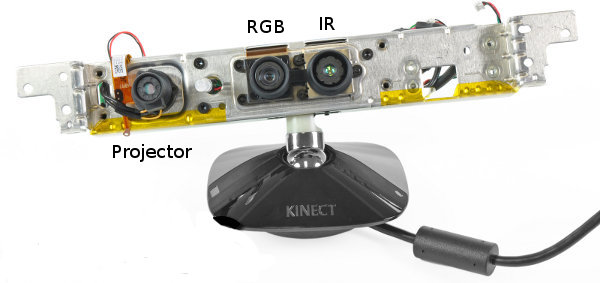
\includegraphics[scale=0.85]{Figures/ros_kinect.jpg}
\decoRule
\caption[Kinect sensor]{Sensor Microsoft Kinect}
\label{fig:Kinect}
\end{figure}

Este sensor salió al mercado a un precio mucho más reducido que algunos que existían antes que él por lo que el interés por este tipo de sensores se disparó y comenzaron a aparecen en diferentes áreas de la tecnología, como interfaces naturales de usuario (en inglés natural user interface, NUI), reconstrucción y realidad virtual o cartografía 3D.

El sensor utilizado en este trabajo es el \textbf{Asus Xtion PRO LIVE} que dispone de la misma tecnología comercializado por Asus, que proporciona profundidad, color y audio (utilizando un micrófono multiarray como el sensor Kinect). \footnote{https://www.asus.com/3D-Sensor/Xtion\_PRO\_LIVE/}

\begin{figure}[th]
\centering
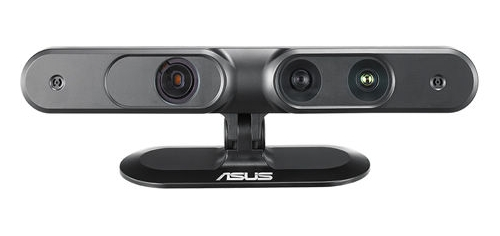
\includegraphics[scale=0.85]{Figures/xtion-pro-live.jpg}
\decoRule
\caption[Kinect sensor]{Asus Xtion PRO LIVE}
\label{fig:Kinect}
\end{figure}


\begin{table}
\caption{Especificaciones técnicas del Asus Xtion PRO LIVE}
\label{tab:xtion}
\centering
\begin{tabular}{ l | l }
\toprule
Campo de visión: & 58º H, 45º V, 70º D\\
\hline
Distancia de uso: & Entre 0.8m y 3.5m\\
\hline
Tamaño de la imagen de profundidad: & VGA (640x480) : 30 fps \\
				& QVGA (320x240): 60 fps\\
\hline
Resolución: & SXGA (1280*1024) \\
\bottomrule
\end{tabular}
\end{table}

Las especificaciones técnicas de este sensor se encuentran recogidas en la tabla ~\ref{tab:xtion}
%----------------------------------------------------------------------------------------
%	SECTION Software
%----------------------------------------------------------------------------------------
%\section{Software}

%-----------------------------------
%	SUBSECTION JDeRobot
%-----------------------------------
\section{JDeRobot}

JDeRobot es un proyecto desarrollado por el grupo de robótica de la Universidad Rey Juan Carlos \footnote{http://jderobot.org}. Consiste en una plataforma de desarrollo de aplicaciones robóticas y de visión artificial. Está en su mayoría escrito en C++, donde disponen de una colección de componentes capaces de comunicarse a través de ICE middleware \footnote{https://zeroc.com/products/ice}, los componentes pueden ejecutarse en diferentes ordenadores y pueden ser programados en diferentes lenguajes.

JdeRobot incluye numerosas herramientas, drivers, interfaces, librerías y tipos. Es \textit{software} libre con licencia GPL y LGPL. También utiliza \textit{software} de terceros como Gazebo, ROS, OpenGL, GTK y Eigen entre otros.

La versión de JdeRobot empleada ha sido la versión 5.4.0. A continuación se detallarán los componentes de JdeRobot que han sido de utilidad para la realización de este proyecto.

\subsection{Biblioteca Progeo}

Es una biblioteca de geometría proyectiva incluida en JdeRobot, que proporciona funciones muy útiles que relacionan puntos en dos y tres dimensiones.

Ha sido realmente útil en este trabajo para que a partir de puntos en dos dimensiones (píxeles) y su correspondiente información de profundidad (distancia), sacar los puntos relativos de la cámara en tres dimensiones.

Progeo usa el modelo de cámara \textbf{Pinhole}, en la Figura~\ref{fig:Pinhole} se puede observar la representación geométrica de la retroproyección y la proyección. Este modelo es definido por unos parámetros intrínsecos y extrínsecos que definen la composición de todos los parámetros iniciales de configuración de la cámara. Los parámetros extrínsecos que establecen la posición 3D, foco de atención (foa) y roll, mientras que los parámetros intrínsecos determinan la distancia focal y el centro óptico o píxel central.

\begin{figure}[th]
\centering
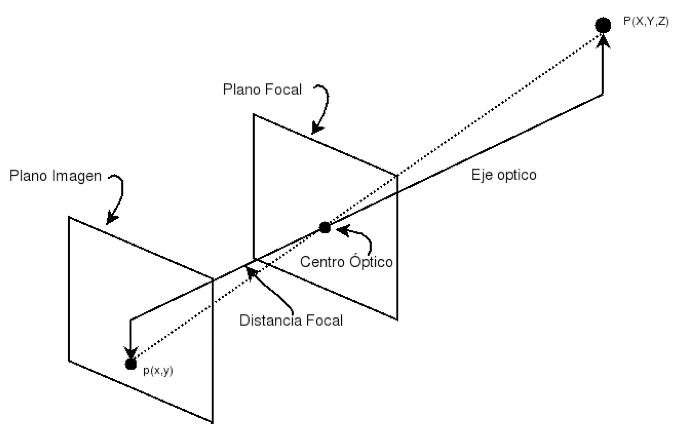
\includegraphics[scale=0.5]{Figures/pinhole-model.jpg}
\decoRule
\caption[pinhole]{Modelo de cámara Pinhole}
\label{fig:Pinhole}
\end{figure}

Las funciones que proporciona esta biblioteca son las siguientes:

\begin{itemize}
\item \textbf{Project}: Esta función permite proyectar un punto 3D del mundo al correspondiente pixel en 2D de la imagen de la cámara. 

\item \textbf{Backproject}: Esta función es capaz de a partir de las coordenadas de un píxel en 2D, obtener la línea de proyección que conecta la cámara y el foco con el rayo 3D que proyecta dicho píxel en el plano imagen. Con esto y conociendo la distancia real del punto 3D a calcular, se calcula las coordenas reales del punto 3D.

\item \textbf{DisplayLine}: Esta función permite conocer si una línea definida por dos puntos en 2D es visible dentro del plano imagen. 

\item \textbf{Display\_info}: Esta función muestra toda la información sobre la cámara utilizada.

\end{itemize}

\subsection{Biblioteca parallelIce}

Es otra librería incluída en JdeRobot, que soluciona el problema de latencia de información proveniente de los diferentes drivers, evitando la espera y proviniendo de un acceso asíncrono a una copia en local de las interfaces con muy bajo tiempo de procesado.

\subsection{Servidor OpenniServer}

OpenniServer es un driver que se comporta como un servidor y es capaz de proporcionar con un sensor RGBD (Kinect o Xtion), imágenes de color, de profundidad o nubes de puntos que son enviados a través de la interfaz ICE a un puerto específico, donde se pueden escuchar los datos. Este driver es el que se necesita para el funcionamiento de este trabajo ya que es desde donde se recogen tanto las imagenes de color (RGB) como las de profundidad (Depth) para su posterior procesado.

\subsection{Herramienta RGBDViewer}

Es una herramienta que permite enseñar la información proveniente de los sensores RGBD con openniServer como forma de visualización de los datos; imágenes RGB, DEPTH o nubes de puntos.

El funcionamiento corresponde a un hilo de ejecución llamado Control que se encarga de recolectar las imágenes provenientes del driver, una clase Shared para guardar y recoger los datos, y por último una clase Gui que se encargará de coger los datos (imágenes y nubes de puntos) guardados en Shared y mostrarlas.

%\begin{figure}[th]
%\centering
%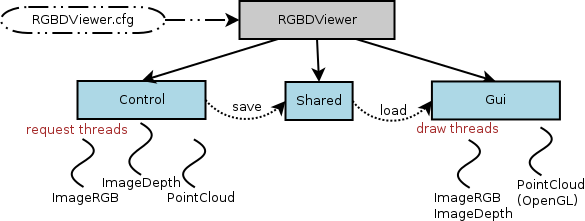
\includegraphics[scale=0.65]{Figures/rgbdviewer.png}
%\decoRule
%\caption[rgbdviewer]{Estructura del funcionamiento de RGBDViewer.}
%\label{fig:RgbdViewer}
%\end{figure}

Esta herramienta a servido como referencia para la realización de este trabajo. En la Figura~\ref{fig:RgbdViewer} podemos ver una captura de pantalla con las diferentes visualizaciones. 

\begin{figure}[th]
\centering
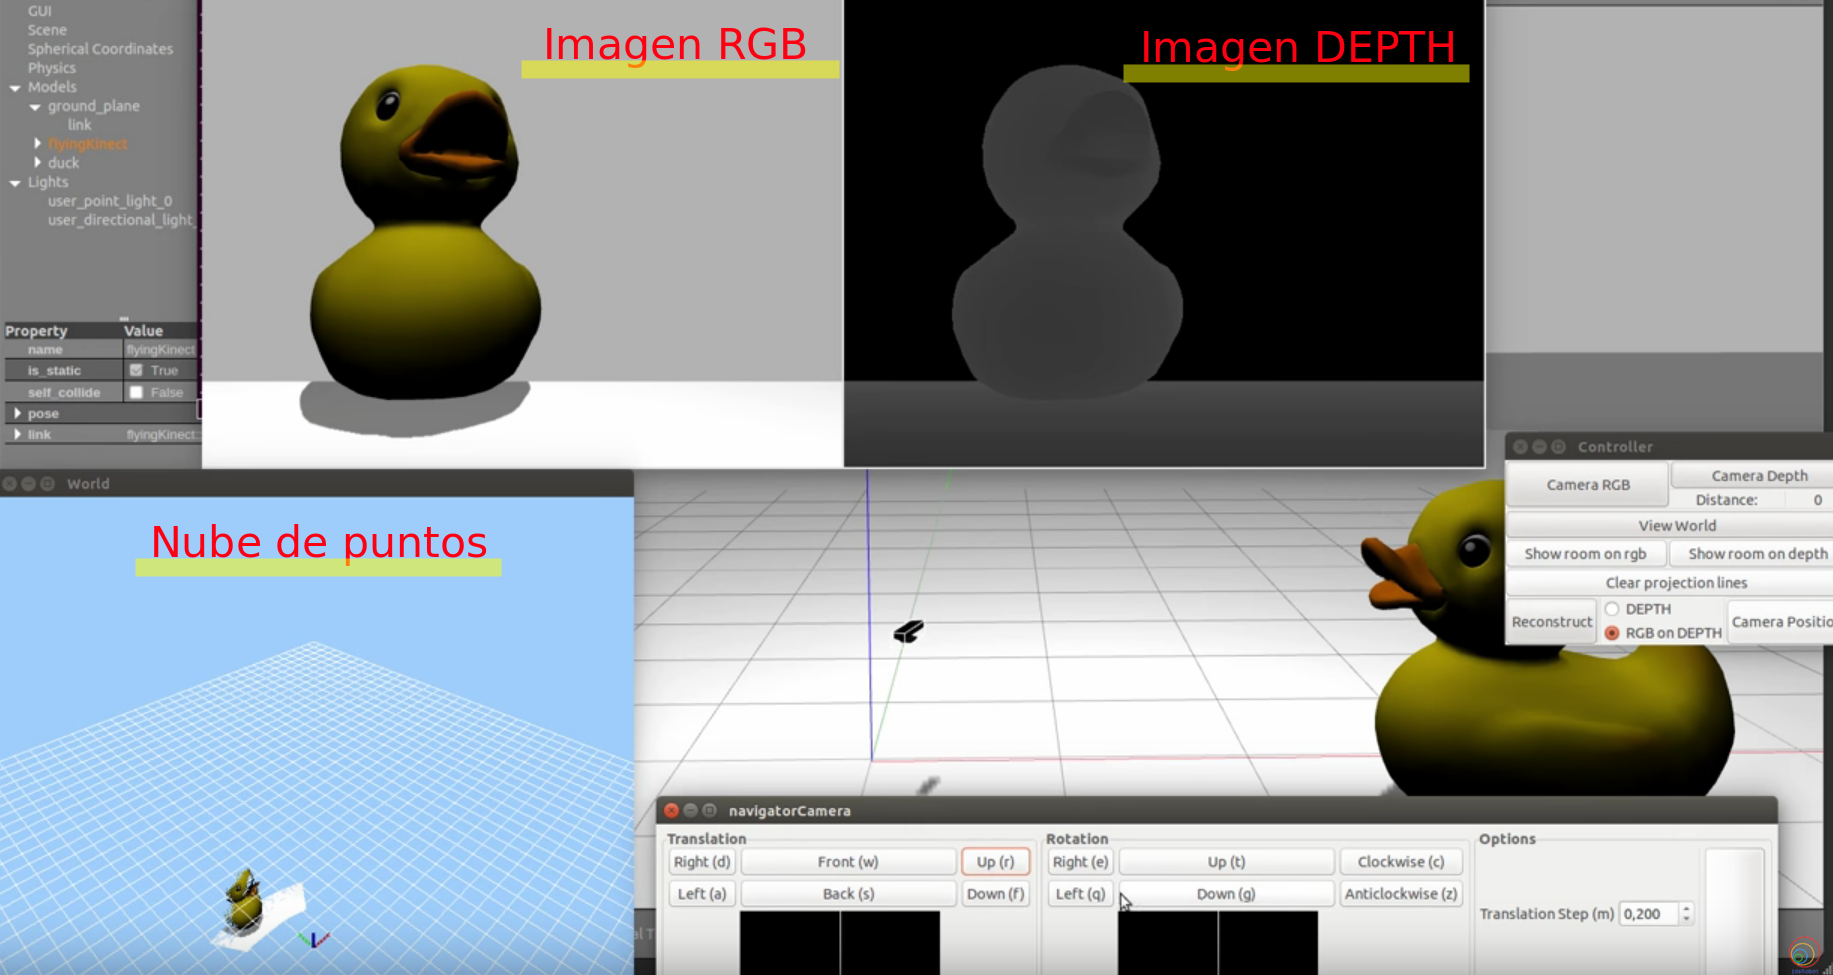
\includegraphics[scale=0.2]{Figures/rgbdviewer2.png}
\decoRule
\caption[rgbdviewer2]{RGBDViewer: Captura de pantalla con las tres vistas de los diferentes datos; imagen de color, de profundidad y nube de puntos.}
\label{fig:RgbdViewer}
\end{figure}

\subsection{Pose3D}

Es una interfaz que define una posición en tres dimensiones (x, y, z, h) y una orientación con un cuaternión (q0, q1, q2, q3).

%\subsection{RGBPoint}

%Es una estructura de datos en la cual se pueden guardar puntos en tres dimensiones con coordenadas (x, y, z), color (r, g, b) y un identificador (id). 
%Para generar las nubes de puntos se ha usado un vector de esta estructura.

%-----------------------------------
%	SUBSECTION ICE
%-----------------------------------
\section{Biblioteca ICE de comunicaciones}

ICE (Internet Communications Engine) es un RPC framework desarrollado por ZeroC con soporte en C++, C\#, Java, JavaScript y Python entre otros. Se encuentra bajo doble licencia GNU GPL y código cerrado. Actúa como plataforma de comunicaciones y funciona bajo TCP/IP. \footnote{https://zeroc.com/products/ice}

En JdeRobot la podemos encontrar como librería y es utilizada como protocolo de comunicaciones entre los diferentes componentes de JdeRobot. En nuestro trabajo se ha usado la versión 3.5.1 y nos ha servido para establecer la comunicación entre el componente y el driver del sensor, recogiendo las imágenes de éste.

%-----------------------------------
%	SUBSECTION PCL
%-----------------------------------
\section{Biblioteca Point Cloud Library (PCL)}

PCL es una librería desarrollada en C++ para el procesamiento de imágenes 2D/3D y nubes de puntos. Está publicada con licencia BSD y libre bajo usos comerciales y de investicación. Está financialmente soportada por un consorcio de companías comerciales y su propia organización sin ánimo de lucro, \textbf{Open Perception}. A parte de los donadores y contribuidores individuales que aportan al proyecto. \footnote{http://pointclouds.org/}

Para simplificar el uso y el desarrollo, esta librería se encuentra dividida en módulos individuales de los que destacan el filtrado de puntos \textit{outliers} o de ruido, estructuras de datos, estimación 3D, algoritmos para la detección de puntos de interés, combinación, segmentación, algoritmos para el reconocimiento de objetos.
%En la Figura~\ref{fig:Grouping} se puede ver un ejemplo de reconicimiento de objetos basado en el módulo pcl\_recognition.

%\begin{figure}[th]
%\centering
%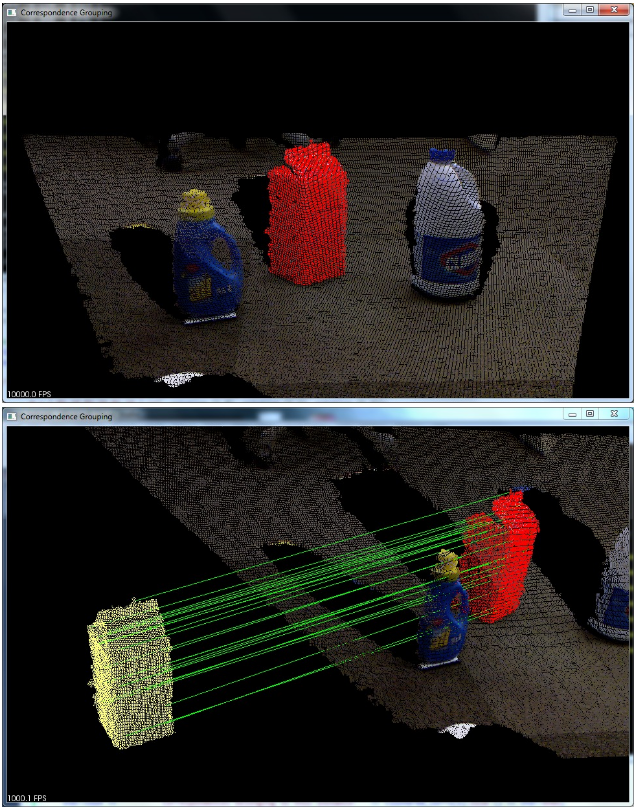
\includegraphics[scale=0.6]{Figures/correspondence_grouping.png}
%\decoRule
%\caption[grouping]{Reconocimiento de objeto 3D con PCL}
%\label{fig:Grouping}
%\end{figure}

En su página web disponen de mucha información y ejemplos prácticos que ayudan mucho a la compresión de todas las funcionalidades de esta librería. PCL también dispone de una librería i/o de entrada y salida para leer o crear nubes de puntos a partir de diferentes dispositivos, así como visualizadores 3D.


%-----------------------------------
%	SUBSECTION OpenCV
%-----------------------------------
\section{Biblioteca OpenCV}

OpenCV (Open Source Computer Vision Library) es una librería de código abierto que fue desarrollada para proporcionar una infraestructura común en aplicaciones de visión artificial y facilitar la inteligencia máquina, con mecanismos de aprendizaje y de interpretación de datos. Con licencia BSD da facilidades para su uso y su modificación bajo fines comerciales. \footnote{http://opencv.org/}

La librería contiene más de 2500 algoritmos. Estos algoritmos pueden ser usados para detectar y reconocer rostros, identificar objetos, clasificar acciones humanas determinadas en vídeos, seguimiento del movimiento de cámaras, seguimiento de objetos, extraer modelos de objetos 3D, producir nubes de puntos a partir de cámaras, encontrar imágenes similares de un conjunto, juntar trozos de imágenes para producir una imagen final con más resolución, etc... OpenCV tiene más de 47 miles de usuarios en la comunidad, excediendo los 14 millones de descargas, la librería es usada ampliamente en empresas, grupos de investigación y organismos gubernamentales.

OpenCV a sido diseñada de forma eficiente y con un fuerte enfoque en aplicaciones de tiempo real. Escrita en C/C++, la librería obtiene las ventajas del procesamiento multi-núcleo. Dispone de interfaces en C++, C, Python, Java y MATLAB y es soportada por diferentes sistemas operativos como Windows, Linux, Android y Mac OS.

En este trabajo se ha utilizado la versión 2.4.8 y se ha usado a la hora de identificar puntos de interés y para los distintos métodos de emparejamiento. En la Figura~\ref{fig:SiftDetector} se puede apreciar un ejemplo de su uso en la detección de puntos de interés sobre un entorno real.

\begin{figure}[th]
\centering
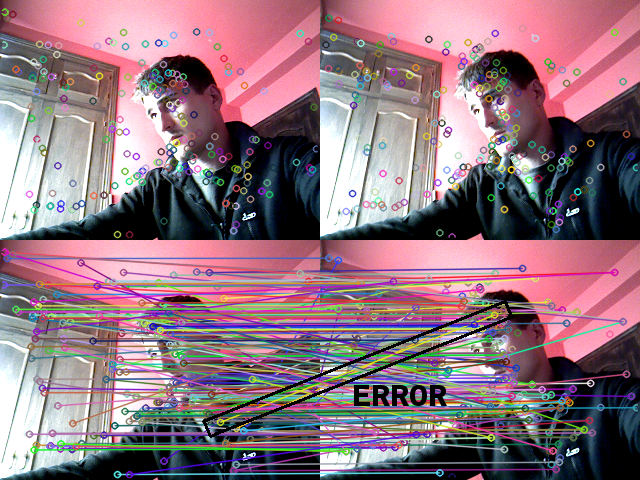
\includegraphics[scale=0.8]{Figures/sift-detector.png}
\decoRule
\caption[sift-detector]{Detección y emparejamiento de puntos de interés con OpenCV usando SIFT.}
\label{fig:SiftDetector}
\end{figure}

%-----------------------------------
%	SUBSECTION Eigen
%-----------------------------------
\section{Biblioteca Eigen}
Eigen es una librería de algebra lineal que permite hacer operaciones aritméticas con matrices y vectores, a través de los operadores comunes de C++, tales como +, -, * o a través de métodos especiales tales como dot(), cross(), etc... Para la clase \textit{Matrix} (matrices y vectores) los operadores solo soportan operaciones de álgebra lineal. En Figura~\ref{fig:Eigen} se puede ver un ejemplo de como de simple es hacer una multiplicación y una división por un escalar. \footnote{http://eigen.tuxfamily.org/}

\begin{figure}[th]
\centering
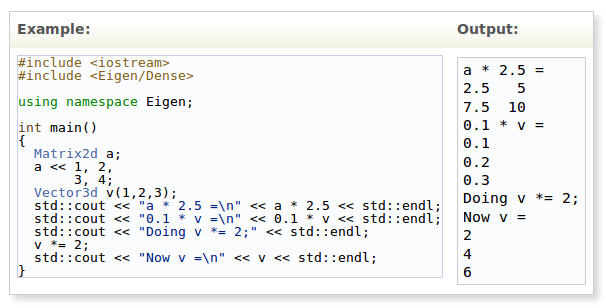
\includegraphics[scale=0.65]{Figures/eigen-multiplication.png}
\decoRule
\caption[eigen]{Ejemplo de una multiplicación y división por un escalar con Eigen.}
\label{fig:Eigen}
\end{figure}

Eigen es \textit{software} libre y desde la versión 3.1.1 tiene licencia MPL2 (LGPL3+ para las anteriores versiones). Se ha usado la versión 3.2.0 y ha sido de utilidad en este proyecto para realizar los cálculos de la matriz RT a través del los vectores de puntos 3D ya emparejados.

%-----------------------------------
%	SUBSECTION GTK
%-----------------------------------
\section{Biblioteca de interfaz gráfica GTK+}
GTK+, o the GIMP Toolkit es una herramienta multiplataforma de creación de interfaces gráficas. Es multiplataforma y está escrito en C, pero a sido diseñado para tener soporte para un gran rango de lenguajes, tales como Perl y Python. GTK++ tiene una gran colección de \textit{widgets} y interfaces para usar en la aplicación, tales como ventanas, botones, selectores, cajas de texto, etc.

La versión utilizada ha sido la 3.10.8. Es \textit{software} libre y parte del proyecto GNU. Con licencia LGPL, permite que sea utilizado por todos los desarrolladores, incluyendo aquellos que están desarrollando un  \textit{software} privativo. GTK+ ha sido utilizado en muchos proyectos y en grandes plataformas. \footnote{https://www.gtk.org/}

\subsection{Glade}
Glade es una \textit{RAD tool} (Rapid Application Development Tool) que permite desarrollar de manera fácil y rápida interfaces de usuario en GTK+ para el entorno de escritorio GNOME. La interfaz gráfica diseñada en Glade es guardada en un XML que usando los objetos GTK+ de \textbf{GtkBuilder} pueden ser cargados y utilizados por aplicaciones de forma dinámica como se ha hecho en este trabajo. \footnote{https://glade.gnome.org/}
%-----------------------------------
%	SUBSECTION OpenGL
%-----------------------------------
\section{OpenGL}
OpenGL es el principal entorno para el desarrollo de aplicaciones gráficas 2D y 3D interactivas. Desde 1992, OpenGL se ha convertido en la interfaz de aplicaciones gráficas más utilizada y soportada en la industria 2D y 3D, con miles de aplicaciones diponibles en diferentes plataformas. OpenGL ayuda al desarrollo de aplicaciones al incorporar un amplio conjunto de renderizado, mapeo de texturas, efectos especiales y otras potentes funciones de visualización. Se puede usar OpenGL en la mayoría de entornos de escritorio y diferentes plataformas. Es muy utilizada y conocida en la industria de los videojuegos.

Algunas de las ventajas de las que presume OpenGL son; que es un estándar de la industria, con soporte, multiplataforma y el único libre. Es estable, dispone de compatibilidad hacia atrás, escalable, fácil de usar y bien documentado. \footnote{https://www.opengl.org/}

Se ha usado la librería \textbf{Mesa 3D Graphics} en linux que es una implementación de la especificación de OpenGL con código abierto \footnote{https://www.mesa3d.org/}.

OpenGL en este trabajo se ha usado para visualizar la posición de la cámara, su estela y la colección de nubes de puntos obtenida y procesada de las imágenes RGB y de profundidad. En la Figura~\ref{fig:OpenGL} se puede apreciar una captura de pantalla con la posición de la cámara dibujada en el espacio tridimensional con el visualizador utilizado con OpenGL.

\begin{figure}[th]
\centering
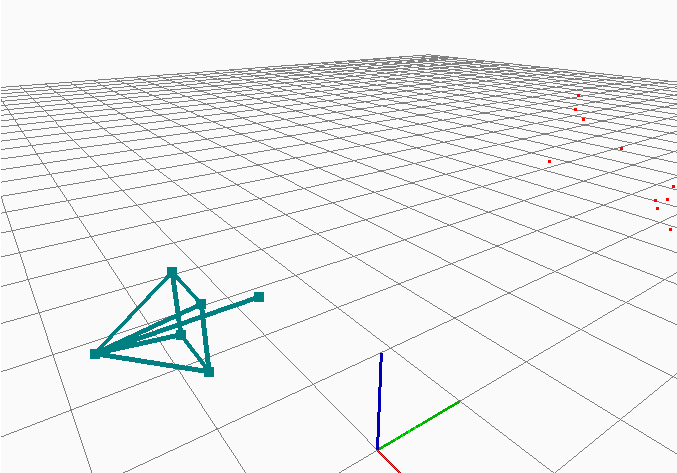
\includegraphics[scale=0.65]{Figures/camera-opengl.png}
\decoRule
\caption[opengl]{Captura de la posición de la cámara en el visualizador 3D con OpenGL.}
\label{fig:OpenGL}
\end{figure}